\chapter{Programming a future universal quantum computer}
%\chapter{Fault-Tolerant Large-Scale Quantum Algorithms?}
% to make contrast with
% Noisy Intermediate-scale Quantum Algorithms?
\label{chpt:programming}

%\epigraph{\textit{Don't believe everything you read on the Internet}}{Abraham Lincoln}
\epigraph{There's plenty of room at the bottom...}{Richard Feynman}

At present, the current power of quantum devices is fundamentally limited by the number of qubits we can engineer in the same physical system. To date, the most qubits achieved on a physical chip is 72 by Google's Bristlecone architecture. However, for a true quantum advantage, most theorise (taking into account the number of qubits required for error correction) that at least one million qubits are required for useful, universal quantum computation. 

From the previous chapter, we learned about useful short-term applications of quantum enhanced computation. These applications, VQE's, adiabatic quantum annealers, will become ever more useful with an increase in resource size, most notably not just simulating the ground states of larger and larger molecules, but also interactions between molecules for catalyst, superconducting material, and drug discovery research.

Aside from increasing resource size for NISQ applications, in the long term increasing the number of error-corrected qubits in a system will allow us to preform much more complex calculations, such as the NP-hard problem of integer factorisation utilising Shor's algorithm, or more efficient unstructured search algorithms via Grover's algorithm. Any problem that can be mapped to these algorithms can benefit from a quantum computational speed-up. 

It is for this reason, that in this section we will be concentrating on the implementation of Shor's and Grover's algorithms (where currently possible) on a multitude of different quantum software platforms. Here we hope to deliver an intuition as to how to program truly useful algorithms on quantum processors in the future.


%%%%%%%%%%%%%%
%%%%%%%%%%%%%%
\begin{comment}
Four (five?) languages will be covered here: 
\begin{itemize}
    \item Quil
    \item QISKit 
    \item Project Q
    \item Q\# (same QDK)
    \item Cirq? anyone?
\end{itemize}

Algorithms to implement:
\begin{itemize}
    \item Grover's algorithm (as example) (Ankur and David have already organised this one, so it'd be nice :3)
    \item Shor's algorithm (as example)
    \item Deutsch's algorithm (as exercise)
\end{itemize}
\end{comment}
%%%%%%%%%%%%%%

\begin{comment}
%%%%%%%%%%%%%%%%%%%%%%%%%%%%%%%
\section{Grover's algorithm} \label{Grover-section}
%%%%%%%%%%%%%%%%%%%%%%%%%%%%%%%


One of the earliest algorithms that was designed to use quantum resources is described in a 1996 paper by Lov Grover \cite{grover1996}. The algorithm attempts to solve the following problem: imagine you have a database of elements. We can represent them as bit strings, but we know that one of them is `marked' by some function acting on that bit string. Examining the case where we have 4 numbers (2 bits), we have the following truth table. 

\begin{equation}
\begin{array}{c|c|c}
    & x & f(x) \\
    \hline
    0 & 00 & 0 \\
    1 & 01 & 0 \\
    2 & 10 & 1 \\
    3 & 11 & 0 \\
\end{array}
\end{equation}

This unstructured search is an important problem in computer science. If we used a classical computer to try to find the marked element `10' above we'd have to try at least 3 times, since we could always end up with it being the last element applied to f(x). This scales as expected, so we can write that at worst it takes N attempts to find the marked element, which can be written O(N).

However, using the principle of superposition, we can explore the whole space of elements simultaneously. To do this we need two matrices (or gates): one which is a diagonal matrix with $(-1)^{f(x)}$ as its elements. For the marked element being 10 as above, we have

\begin{align}
        U_f = \begin{pmatrix}
        1 & 0 & 0 & 0 \\
                 0 & 1 & 0 & 0\\
                 0  & 0 & -1 & 0 \\
                 0 & 0 & 0 & 1
        \end{pmatrix}
\end{align}

The second ingredient is the following matrix, (irrespective of which element is marked).

\begin{align}
        D = \frac{1}{2}\begin{pmatrix}
        -1 & 1 & 1 & 1 \\
                 1 & -1 & 1 & 1\\
                 1  & 1 & -1 & 1 \\
                 1 & 1 & 1 & -1
        \end{pmatrix}
\end{align}

Now we will look at the algorithm step-by-step for this simple four element (two qubit) case. Starting with the qubits in the `00` state, we generate a superposition using a so called Hadamard gate (represented by H) on each qubit, which takes $00 \rightarrow 00 + 01 + 10 +11$ (we have ignored normalisation for simplicity). This can be represented by the matrix transformation

\begin{align}
        \frac{1}{2}
        \begin{pmatrix}
        1 & 1 & 1 & 1 \\
        1 & -1 & 1 & -1\\
        1  & 1 & -1 & -1 \\
        1 & -1 & -1 & 1
        \end{pmatrix}
        \begin{pmatrix}
        1\\
        0\\
        0\\
        0\\
        \end{pmatrix}
        =
        \frac{1}{2}
        \begin{pmatrix}
        1\\
        1\\
        1\\
        1\\
        \end{pmatrix}
\end{align}

In the next step of the algorithm, we apply $U_f$. This picks out the marked element, giving it a minus sign and adding a $\pi$ phase shift to the other elements.

\begin{align}
        \frac{1}{2}
        \begin{pmatrix}
        1 & 0 & 0 & 0 \\
        0 & 1 & 0 & 0\\
        0  & 0 & -1 & 0 \\
        0 & 0 & 0 & 1
        \end{pmatrix}
        \begin{pmatrix}
        1\\
        1\\
        1\\
        1\\
        \end{pmatrix}
        =
        \frac{1}{2}
        \begin{pmatrix}
        1\\
        1\\
        -1\\
        1\\
        \end{pmatrix}
\end{align}

The final step is to apply $D$. The construction is $D$ is such that each row, when multiplied by the vector, converts the $\pi$ phase difference into unit value . This can be thought of as a constructive interference on the marked element instead of destructive interference on all of the other elements. 

\begin{align}
    \frac{1}{2}.\frac{1}{2}
    \begin{pmatrix}
    -1 & 1 & 1 & 1\\
    1 & -1 & 1 & 1 \\
    1 & 1 & -1 & 1 \\
    1 & -1 & -1 & 1 \\
    \end{pmatrix}
    \begin{pmatrix}
    1 \\ 1 \\ -1 \\ 1 
    \end{pmatrix}
    =
    \frac{1}{4}
    \begin{pmatrix}
    0 \\ 0 \\ 4 \\ 0
    \end{pmatrix}
    = 
    \begin{pmatrix}
    0 \\ 0 \\ 1 \\ 0
    \end{pmatrix}
\end{align}

From this we can see that the general recipe of Grover's algorithm is to create a superposition of all the possible states, add a $\pi$ phase shift to the marked states with the special unitary $U_f$, and then use $D$ to pick out this phase shift.

In this case the algorithm has successfully found the marked element with certainty (though this does not take into account any experimental imperfections observed in real life). However, using superpositions inevitably leads to success with a non-unity success rate, as demonstrated in the next section, where we look at the three qubit case described using Dirac notation instead of matrices, as now we would have to use $8\times8$ matrices - this demonstrates the exponential scaling that quantum computing demonstrates, with $2^n\times2^n$ matrices being required for $n$ qubits. Hence the transition to Dirac notation is quite a natural progression to larger system sizes. 

%%%%%%%%%%%%%%%%%%%%%%%%%%%%%%%%%%%%%%%%%
\subsubsection{Alternative representation: Dirac notation}
Here we consider a problem on $N=8$ elements, where the fifth element is marked. The algorithm can be applied with a minimum of $3$  ($2^{3}=8$) qubits in the following manner:

\begin{tcolorbox}[standard jigsaw,
    opacityback=0,  % this works only in combination with the key "standard jigsaw"
    boxrule=0.5pt,label={example100100000}]
    {\bf Grover's Algorithm}
    \tcbline
    \begin{enumerate}
    \item Start with the state $\ket{000}$.
    \item Apply the Hadamard gates which result in the state: $\ket{\Psi}=\dfrac{1}{2\sqrt{2}}\big(\ket{000}+\ket{001}+\ket{010}+\ket{011}+\ket{100}+\ket{101}+\ket{110}+\ket{111}\big)$
    \item Apply $U_{f}$, which reverses the sign on the fifth element: $\ket{\Psi}=\dfrac{1}{2\sqrt{2}}\big(\ket{000}+\ket{001}+\ket{010}+\ket{011}-\ket{100}+\ket{101}+\ket{110}+\ket{111}\big)$
    \item Apply D, which leads to state $\ket{\Psi}=\dfrac{1}{4\sqrt{2}}\big(\ket{000}+\ket{001}+\ket{010}+\ket{011}+5\ket{100}+\ket{101}+\ket{110}+\ket{111}\big)$
    \item Repeat steps 3 and 4 ``$T$'' times, where $T$ is to be determined later.
    \item Measure the state $\ket{\Psi}$.
    \end{enumerate}
\end{tcolorbox}



\begin{figure}
    \centering
    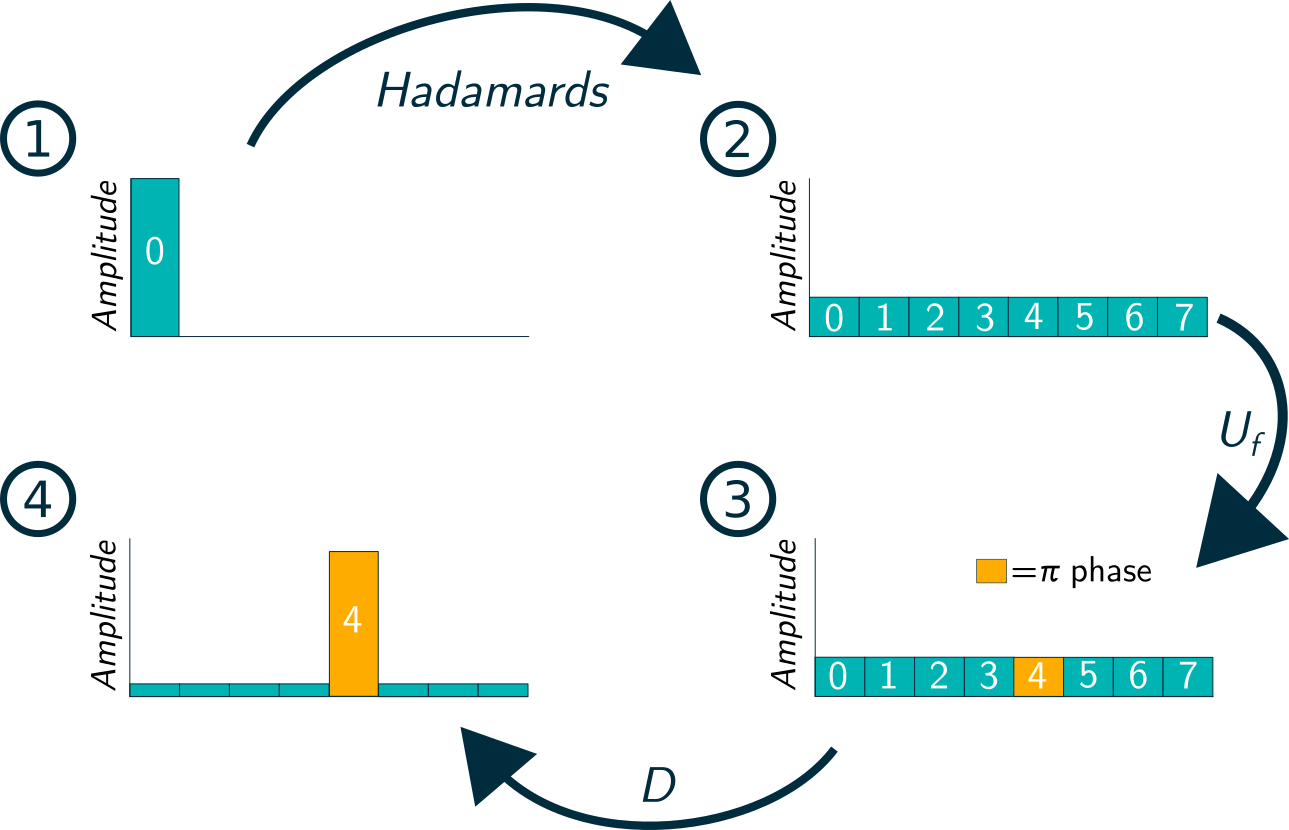
\includegraphics[width=0.9\linewidth]{figures/Grovers.png}
    \caption{Pictorial demonstration of the steps of Grover's Algorithm}
    \label{fig:Grovers}
\end{figure}


In the step 2 above, applying the Hadamard gate to all the qubits leads to a state which is in superposition of all possible states (elements). It is important to start with the state $\ket{000}$ so that all the states in the superposition have the same initial phase. In step 3 we apply the $U_{f}$ gate which is dependent on $f(x)$ and is able to recognise the marked element. The oracle applies a $\pi$ phase shift to the marked element but leaves all the other states unchanged. The next step is to apply gate $D$. The application of gate $D$ can be understood as an operation which increases the amplitude of the phase shifted element in step 3, suppressing the amplitude of the others. As mentioned in chapter 1, the measurement of a state leads to an output with a probability equal to the amplitude squared and thus, increasing the amplitude of the marked element state results in a higher probability of a measuring returning that state. It is worth noting that repeating steps 3 and 4 a fixed number of times will increase the probability of detecting the marked element but after a certain point, the probability will start to decrease. For clarification, if we carry out another iteration of steps 3 and 4 in the above example, we get the state:
\begin{align}
\ket{\Psi}=\dfrac{-1}{8\sqrt{2}}\big(\ket{000}+\ket{001}+\ket{010}+\ket{011}-11\ket{100}+\ket{101}+\ket{110}+\ket{111}\big).
\end{align}
 Now if a measurement is performed on this state, there is a 94.53\% chance of getting the fifth element compared to 78.12\% probability after just one iteration. If yet another iteration of step 3 and 4 is performed, the resulting state becomes:

\begin{align}
\ket{\Psi}=\dfrac{-7}{16\sqrt{2}}\big(\ket{000}+\ket{001}+\ket{010}+\ket{011}-\frac{13}{7}\ket{100}+\ket{101}+\ket{110}+\ket{111}\big)    
\end{align}
and the probability of getting the marked element upon measurement decreases further to 67\%. Therefore, it is important to choose the number of iterations for Grover's algorithm carefully. The number of iterations ``$T$'' required to get the maximum probability of measuring the marked element is approximately given by:

\begin{equation}\label{groverIteration}
    T=\big(\pi\big/4)\sqrt{N}
\end{equation}


%%%%%%%%%%%%%%%%%%%%%%%%%%%%%%%%%%%%
\subsubsection{General n-qubit case}

Given a function $f: \left\{0,1\right\}^n \rightarrow \left\{0,1\right\}$ with the promise that $f(x_0) = 1$ for a unique element $x_0$, the problem is to find this $x_0$. We use a quantum circuit on $n$ qubits in the initial state $\ket{0}^{\otimes n}$. Let $H$ denote the Hadamard gate, and let $U_0$ denote the $n$-qubit operation which inverts the phase of $\ket{0^n}$: $U_0\ket{0^n} = -\ket{0^n}$, $U_0\ket{x} = \ket{x}$ for all $x \neq 0^n$. The first step of the algorithm is to apply the Hadamard gate on all $n$ qubits to form the superposition state required for quantum parallel computing. Next, repeat the following operations T times for some T determined by Equation \ref{groverIteration}.
%\begin{enumerate}
%\item Apply $H^{\otimes n}$.

%\item Repeat the following operations T times, for some T to be determined later:
\begin{enumerate}
\item Apply $U_f$, where $U_f\ket{x} = (-1)^{f(x)}\ket{x}$.
\item Apply $D$, where $D = -H^{\otimes n}U_0H^{\otimes n}$
\end{enumerate} 
%\item Measure all the qubits and output the result.
%\end{enumerate}
%\end{tcolorbox}
Finally, measure all the qubits and output the result.\\

In circuit diagram form, Grover's algorithm appears like: \\
\begin{equation*}
\Qcircuit @C=2.14em @R=1.25em
{\lstick{\ket{0}} & \gate{H} & \multigate{5}{U_f} & \multigate{5}{D} & \multigate{5}{U_f} & \ghost{U_f} & \lstick{\dots} & \multigate{5}{D} & \meter \\
\lstick{\ket{0}} & \gate{H} & \ghost{U_f} & \ghost{D} & \ghost{U_f} & \ghost{U_f} &\lstick{\dots} & \ghost{D} & \meter \\ 
& \dot{} & & & & & & & \dot{} \\
& \dot{} & & & & & & & \dot{} \\
& \dot{} & & & & & & & \dot{} \\
\lstick{\ket{0}} & \gate{H} & \ghost{U_f} & \ghost{D} & \ghost{U_f} & \ghost{U_f} & \lstick{\dots} & \ghost{D} & \meter \\}
\end{equation*}

\subsubsection{Construction of gate $D$ and $U_{f}$}
The gate $D$ in the algorithm applied on $n$-qubits can be implemented in the following manner. This shows that gate $D$ requires $2n+1$ Hadamard ($H$) gates, $2n+1$ Pauli $X$ gates and an n-control Toffoli gate.

\begin{align*}
\Qcircuit @C=1.14em @R=1.25em
{\lstick{\ket{x_1}} & \gate{H} & \gate{X} &  \ctrl{1} & \gate{X} & \gate{H} & \qw  \\
\lstick{\ket{x_2}} & \gate{H} & \gate{X} &  \ctrl{4} & \gate{X} & \gate{H} & \qw  \\
\lstick{\dot{}} & \dot{} & \dot{} & & \dot{} & \dot{} & \\
\lstick{\dot{}} & \dot{} & \dot{} & & \dot{} & \dot{} & \\
\lstick{\dot{}} & \dot{} & \dot{} & & \dot{} & \dot{} & \\
\lstick{\ket{x_n}} & \gate{H} & \gate{X} &  \ctrl{1} & \gate{X} & \gate{H} & \qw  \\
\lstick{\ket{0}} & \gate{x} & \gate{H} &  \targ & \qw & \qw & \qw }
\end{align*}

\vspace{1cm}
The construction of gate $U_{f}$ depends upon the function $f(x)$ being addressed by the algorithm.

\end{comment}
%%%%%%%%%%%%%%%%%%%%%%%%%%%%%%%%%%%%%%%%%
\section{Implementing Grover's algorithm}
%%%%%%%%%%%%%%%%%%%%%%%%%%%%%%%%%%%%%%%%%

In this section we will implement Grover's algorithm as discussed in \autoref{Grover-section}. The steps that we need to implement Grover's algorithm are as follows

\begin{enumerate}
    \item{Import/initialise libraries}
    \item{Create the equal superposition}
    \item{Define the oracle operations $U_f$ and $D$ described in \autoref{Grover-section} }
    \item{Perform the oracle operations T times}
    \item{Measure the register to obtain the output}
\end{enumerate}

For our implementations the unique bit string to be found is given by either the user or a random number generator, rather than being given a black box with a single marked element. Therefore this just serves as a simple example for how Grover's algorithm will work.

We will aim to discuss the most important sections of the code which are the quantum parts. For the full code listings please check out our Appendix/Github.

%%%%%%%%%%%%%%%%%%%%%%%%%%%%%%%%%%%%%%%%%%%
%%%%%%%%%%%%%%%%%%%%%%%%%%%%%%%%%%%%%%%%%%%
\subsection{Grover's Algorithm with pyQuil}
%%%%%%%%%%%%%%%%%%%%%%%%%%%%%%%%%%%%%%%%%%%
%%%%%%%%%%%%%%%%%%%%%%%%%%%%%%%%%%%%%%%%%%%

\subsubsection{Initialise libraries}

We start by calling the libraries that we are going to use

\inputminted[lastline=5]{python}{code/pyQuil/grover_pyquil_guide.txt}

and initialise the program

\inputminted[firstnumber=18, firstline=18, lastline=20]{python}{code/pyQuil/grover_pyquil_guide.txt}

\subsubsection{Create the equal superposition}

We can create the equal superposition by looping through all of the qubits and applying a Hadamard to each of them.

\inputminted[firstnumber=22, firstline=22, lastline=24]{python}{code/pyQuil/grover_pyquil_guide.txt}

\subsubsection{Create the oracle operations}

Defining the Oracles matrices and adding them to be gates
\begin{minted}[firstnumber=17]{python}
# Defining Oracle matrices: U0 and Uf
vec0=np.ones((2**n,), dtype=np.int)
vecf=np.ones((2**n,), dtype=np.int)
vec0[0]=vec0[0]*(-1)
vecf[nf]=vecf[nf]*(-1)
U0ma=(-1)*np.diag(vec0) 
Ufma=np.diag(vecf) 
# Defining Oracle gates
p.defgate("U0",U0ma)
p.defgate("Uf",Ufma)
\end{minted}

\subsubsection{Apply the oracle operations}

Calculating T and applying the operator of interest T times.
\begin{minted}[firstnumber=27]{python}
# Calculating T for the loop
T=((np.pi/4)*(1/np.arcsin(1/np.sqrt(2**n))))-0.5 # N=2**n
T=np.rint(T)
T=int(T)
# Applying Oracle loop T times
for i in range(1,T+1,1):
    p.inst(("Uf",)+tuple(range(n)))
    for ii in range(0, n, 1):
        p.inst(H(ii))
    p.inst(("U0",)+tuple(range(n)))
    for ii in range(0, n, 1):
        p.inst(H(ii))
\end{minted}

\subsubsection{Measure the register to obtain the output}

Measuring all the qubits and running the program.
\begin{minted}[firstnumber=39]{python}
# Measurement stage
for ii in range(0, n, 1):
    p.measure(ii,ii)
# Running the program
results=qvm.run(p,[],5)
guess=results[0]
print("""Grover's algorithm is guessing that the marked string is""",guess)
\end{minted}
The algorithm ends up printing a guess for the single-marked string.

%Define it as a function, so that if u run the algorithm it outputs this and that.

%%%%%%%%%%%%%%%%%%%%%%%%%%%%%%%%%%%%%%%%%%%
\subsection{Grover's Algorithm with QISKit}

\subsubsection{Initialise libraries}

Firstly, as with most regular programming languages, we need to import the libraries that we intend to make use of:

\begin{minted}{python}
# Program written using QISKit to demonstrate the way in which to implement Grovers search 
# algorithm and then simulate the measurement on IBM's Q QASM simulator

# Import relevant library functions from QISKit
from qiskit import ClassicalRegister, QuantumRegister, QuantumCircuit, QuantumProgram
from qiskit import available_backends, execute

# Import relevant library functions 
import numpy as np
\end{minted}

Here we define out function, the length of the marked element inputted by the user, the length of said marked element, and the number of qubits required to preform a search algorithm that will find said marked element:

\begin{minted}[firstnumber=10]{python}
def grover(marked_element):
	
	# Determine the number of qubits needed
	n = len(marked_element)
	N = 2**n
	print('Number of Qubits required is', n)
	print('Number of Ancillas required is', n)
\end{minted}

Due to the way in which QISKit handles inputted strings, for the output of our function to make sense it is necessary to flip the values of the use inputted bit string:

\begin{minted}[firstnumber=17]{python}	
	# Flip bitstring
	marked_element = marked_element[::-1]
\end{minted}

Here we add in protection against user input that would require too many qubits to execute successfully. Via QISKit's local Q QASM simulator, we have the equivalent of 32 qubits available to us to preform simulations. In these lines the function returns 0 is the used input requires more than 32 qubits:

\begin{minted}[firstnumber=19]{python}	
	# Check if we can simulate on our local simulator (QASM Local simulator has 32 
	# qubits)
	if n > 32:
		print('Number of qubits required =', 2*n, 'which is too large to simulate.')
		return 0
\end{minted}

The code here shows how we calculate the number of iterations necessary to identify the user inputted bit string:

\begin{minted}[firstnumber=24]{python}	
	# Determine the number of times to iterate 
	T = int(round(np.pi*np.sqrt(N)/4 - 0.5)) 
	print('Number of iterations T =',T)
\end{minted}

Now comes the QISKit element. Below we show how to define our $n$-qubit register, an $n+1$ classical readout register, $n-1$ ancilla qubits for two qubit operations, and a target register to aid in the implementation of an $n$-qubit CNOT gate. We then combine all of these resources into a single quantum circuit we can manipulate:

\begin{minted}[firstnumber=27]{python}
	# Initialise n qubit register, classical readout register and ancilla qubit
	q = QuantumRegister(n, 'ctrl')
	c = ClassicalRegister(n+1, 'meas')
	a = QuantumRegister(n-1, 'anc')
	t = QuantumRegister(1, 'tgt')
	
	# Combine resources into a quantum circuit
	qc = QuantumCircuit(q, a, t, c)
\end{minted}

\subsubsection{Create the equal superposition}

Here we manipulate entire registers by looping through and applying unitary gates to each qubit in the register:

\begin{minted}[firstnumber=35]{python}
	# Step 1: Start in an equal weighted superposition state on the quantum register 
	for i in range(n):
		qc.h(q[i])
	
	# Put the ancilla qubit into the - state
	qc.x(a[0])
	qc.h(a[0])
\end{minted}

\subsubsection{Apply the oracle operations}

From any quantum computation literature it is known that to execute Grover's successfully, the operations $D$ and $U_{f}$ must be repeated sequentially $T$ times. This is shown in the framework of QISKit below:

\begin{minted}[firstnumber=42]{python}	
	# Step 2: Repeat applications of U_f and D
	for i in range(T):
		# Apply U_f 
		for j in range(n):
			if marked_element[j] == '0':
				qc.x(q[j])	
		
		# Implement an n-qubit CNOT gate
		qc.ccx(q[0], q[1], a[0])
		for i in range(2, n):
			qc.ccx(q[i], a[i-2], a[i-1])
		# Copy
		qc.cx(a[n-2], t[0])
		# Uncompute
		for i in range(n-1, 1, -1):
			qc.ccx(q[i], a[i-2], a[i-1])
		qc.ccx(q[0], q[1], a[0])
		
		for j in range(n):
			if marked_element[j] == '0':
				qc.x(q[j])
		
		# Apply D
		
		# Apply H
		for j in range(n):
			qc.h(q[j])
			qc.x(q[j])
		
		# Apply U_0
		# Implement an n-qubit CNOT gate
		qc.ccx(q[0], q[1], a[0])
		for i in range(2, n):
			qc.ccx(q[i], a[i-2], a[i-1])
                # Copy
		qc.cx(a[n-2], t[0])
                # Uncompute
		for i in range(n-1, 1, -1):
			qc.ccx(q[i], a[i-2], a[i-1])
		qc.ccx(q[0], q[1], a[0])
		
		# Apply H
		for j in range(n):
			qc.x(q[j])
			qc.h(q[j])
\end{minted}

\subsubsection{Measure the register to obtain the output}

Coming to the end of the program, we 'measure' our quantum register onto a classical register:

\begin{minted}[firstnumber=87]{python}	
		# Measure our quantum register via our classical register
		for i in range(n):
			qc.measure(q[i], c[i])
\end{minted}

Finally, we execute our program on the local Q QASM simulator:

\begin{minted}[firstnumber=90]{python}
		# Execute the quantum circuit on the local simulator
		job = execute(qc, 'local_qasm_simulator')
		result = job.result()
		print('The results of the simulation shots are:', result.get_counts(qc))
\end{minted}

Here we end the function by defining what type of input the user can submit to the function we just defined:

\begin{minted}[firstnumber=94]{python}
# Define input type for def
str_input = input("Input a bit string to find: ")
grover(str_input) 
\end{minted}

%%%%%%%%%%%%%%%%%%%%%%%%%%%%%%%%%%%%%%%%%%%
\subsection{Grover's Algorithm with ProjectQ}
%%%%%%%%%%%%%%%%%%%%%%%%%%%%%%%%%%%%%%%%%%%

The first thing to do is to import the functions from ProjectQ that will be required to create and run the program.

\inputminted[firstnumber=3, firstline=3, lastline=5]{python}{code/ProjectQ/grover_projectq_guide.txt}

Since ProjectQ is run on a local simulator, your computer, it is good practice to make sure that the number of qubits required for the computation can actually be simulated to avoid crashing the computer. Most modern computers have 8GB of RAM which is exactly enough memory for 29 qubits, but there are other processes being run on the computer so you would only be able to simulate 28.

\inputminted[firstnumber=13, firstline= 13, lastline=16]{python}{code/ProjectQ/grover_projectq_guide.txt}

Now the local simulator can be loaded by calling \texttt{MainEngine} and our qubits allocated. The number of qubits required is the length of the bit string provided by the user plus an ancilla qubit. The ancilla is required because we will use it to implement the oracle $U_f$ and the gate $D$.

\inputminted[firstnumber=22, firstline=22, lastline=25]{python}{code/ProjectQ/grover_projectq_guide.txt}

The main qubits need to start in an equal superposition, so Hadamards can be applied to all of them using the function \texttt{All}. The ancilla needs to start in the $\ket{-}$ state, and since qubits are initialised as $\ket{0}$, we can achieve this with an $X$ followed by a $H$ gate.

\inputminted[firstnumber=27, firstline=27, lastline=30]{python}{code/ProjectQ/grover_projectq_guide.txt}

Now we come to the part of the algorithm where we must alternate between the gates $U_f$ and $D$ for $T$ iterations where $T$ is the closest integer to $\frac{\pi}{4}\sqrt{N} - \frac{1}{2}$. ProjectQ does allow you to define new gates from their matrix representations using \texttt{BasicGate}, but this only works well for one or two qubit gates. Therefore we need a different, more efficient way of doing the oracle. 

To perform $U_f$, we can use the function \texttt{Control} from ProjectQ. This controls on all the qubits being in the state $\ket{1}$ - so it essentially functions as a quantum \texttt{if} statement. Suppose that the marked bit string is '101', $U_f$ should flip the phase of $\ket{101}$. But since we can only control on all the bits being '1', we need to flip the second bit using an $X$ gate. Once we have done this, we can use an $X$ gate on the ancilla to introduce this phase, then flip the second bit back to normal. Our code can now generalise to any bit string.

\inputminted[firstnumber=34, firstline=34, lastline=42]{python}{code/ProjectQ/grover_projectq_guide.txt}

Now we can do a similar construction to implement the gate $D = H^{\otimes n} U_0 H^{\otimes n}$. This time flipping all the qubits with $X$ since we need to control on all the qubits being $\ket{0}$. 

\inputminted[firstnumber=43, firstline=43, lastline=52]{python}{code/ProjectQ/grover_projectq_guide.txt}

Finally, after we exit the loop, we must measure all the qubits using the \texttt{Measure} command and use \texttt{flush} to send all the instructions to the simulator. The result can then be converted to an integer from a qubit type using \texttt{int} and displayed as a string.

\inputminted[firstnumber=54, firstline=54, lastline=59]{python}{code/ProjectQ/grover_projectq_guide.txt}

An example of the input and output is shown below. Up until around 16 qubits, the code takes less than a minute to run. Beyond that, not only do we have more qubits to simulate, but we also have to apply more gates as the number of iterations required increases. For example, trying to find a 20-bit string takes around 30 minutes.

\begin{minted}{python}
Input a bit string to find: 10101
Number of iterations T = 4
Element found = 10101
\end{minted}

%%%%%%%%%%%%%%%%%%%%%%%%%%%%%%%%%%%%%%%%%%%%
\subsection{Grover's Algorithm with Q\#}

We start Grover's algorithm as any other Q\# program, by declaring the namespace we are working in, \texttt{Quantum.Grover} and open the namespaces we will be using.

\lstinputlisting[language=Qsharp, firstnumber=1, linerange={1-7,127-127}]{code/Qsharp/Grover/Grover.txt}

Programming quantum algorithms

When implementing a quantum program, an important step is to check the individual gates that are required for the program and ensure you know how to program them. In the case of Grover's algorithm we need various gates: first of all we need the Hadamard ($H$) gate, which is a primitive gate and provided by Q\#. The other two main gates are more complex. $U_f$, the phase oracle dependent on the function $f(x)$ which marks the element we search for with Grover's and the gate $D = H^{\otimes n} U_0 H^{\otimes n}$ are not standard gates in Q\# and will need to be coded up. Both operations require phase oracles. One can implement these using a bit oracle and an additional qubit, the ancilla qubit.

Let us have a look at the operation $U_f$, the general phase oracle. The operation takes three inputs: the main register of qubits \texttt{reg}, the ancilla qubit \texttt{ancilla} and the marked element in this search in a bit string equivalent representation \texttt{markedElement}.
To implement the phase oracle with a bit oracle we then simply apply a NOT ($X$) gate on the ancilla controlled on the main register being in the marked state.

Q\# has a build in mechanism to allow controlled operations. Using the syntax \texttt{(Controlled Operation)([ctrl], (arg1, arg2, ...))} one can ensure that operation \texttt{Operation} is controlled by all qubits in \texttt{Qubit[] ctrl} and receives the required arguments \texttt{arg1}, etc. However, the controlled operation is always selected on the $\ket{11...1}$ state, which is why we flip all states in the register where the bit string of the marked element is zero.

To ensure that we exit the operation having only changed the ancilla qubit, we have to flip those qubits in the main register back that we flipped before the controlled NOT on the ancilla.

However, with just defining the body of the operation we are not yet done. As this operation does not contain any measuring operations, it can be easily inverted, creating the so-called "adjoint" operation. This can be done simply with the statement \texttt{adjoint auto}. Similarly, we can create a controlled version of the operation with \texttt{controlled auto}, as all basic operation are controllable, too, and even the controlled inverted equivalent with \texttt{controlled adjoint auto}. This allows the operation to be used in four different ways with writing just one implementation. 

%\inputminted[firstline=67,lastline=93]{csharp}{code/Qsharp/Grover/Grover.txt}

\lstinputlisting[language=Qsharp, firstnumber=67, linerange={67-93}]{code/Qsharp/Grover/Grover.txt}

Next we implement the $D$ operation. We start with applying the Hadamard to every bit in the main register, using the library function \texttt{ApplyToEachCA}. This applies a one qubit operation to every qubit in the given register. The "CA" at the end indicates that this function is the controllable and adjointable version, so we can make the operation \texttt{D} controllable and adjointable again.

Then we perform $U_0$, in this case a controlled NOT ($X$) gate on the ancilla selecting on the $\ket{00..0}$ state by flipping all qubits in the main register. After flipping all these back, we perform the Hadamard again on all qubits as the last step of $D$.

\lstinputlisting[language=Qsharp, firstnumber=95, linerange={95-114}]{code/Qsharp/Grover/Grover.txt}

Now we have all the elements we need to implement Grover's algorithm. We start by calculating the length of the qubit register we will need and creating a random number that will represent the marked element and the integer array form that our $U_f$ requires.

The bit string representation is in so-called little-endian form. Endianness is concerned with which (qu)bit is the most significant: e.g. if \texttt{01} means $0\times2^0+1\times2^1 = 2$ or $0\times2^1+1\times2^0 = 1$. In the first case the first (qu)bit represents the smallest value, which is also denoted "little-endian". The second case gives the largest, i.e. most significant value, first, so it is also called "big-endian". Q\# has various operations which use either of these orderings, which will be important in the implementation of Shor's algorithm.

\lstinputlisting[language=Qsharp, firstnumber=8, linerange={8-23}]{code/Qsharp/Grover/Grover.txt}

Next we allocate the qubits we will use with a \texttt{using} statement, where we allocate the main register and the ancilla together. Next we have to split these into two arrays, the main register \texttt{reg} and the ancilla qubit \texttt{ancilla}.
On a side note: the variable \texttt{outcome} will hold the result of the quantum algorithm. It needs to be declared outside the \texttt{using} block, as all variable declared inside the block are local and the return statement, which must be outside the block, otherwise cannot access it.

\lstinputlisting[language=Qsharp, firstnumber=28, linerange={28-39}]{code/Qsharp/Grover/Grover.txt}

Now we can start implementing the algorithm. We apply the Hadamard to all qubits in the main register and set the ancilla qubit to the required $\ket{-}$ state. Note that we use a different version of the \texttt{ApplyToEach} operation here. As we are in the main operation, which also contains measurements, we do not have to worry about the operation being adjointable or controllable. 

Next we apply the $U_f$ and $D$ operations $T = \frac{\pi}{4}\sqrt{N}$ times to get to the required state and finally we measure the main register to find the marked element with high probability.

\lstinputlisting[language=Qsharp, firstnumber=41, linerange={41-56}]{code/Qsharp/Grover/Grover.txt}

The last steps of the operation are cleaning the qubits with the \texttt{ResetAll} operation, i.e. set them all back to the $\ket{0}$ state, and releasing them by exiting the \texttt{using} block. Cleaning qubits is good practise and should always be done before releasing the qubits you used. Finally, we return both the measured outcome of the quantum algorithm and the marked element we randomly chose in the beginning to allow the user to check if the algorithm worked. 

\lstinputlisting[language=Qsharp, firstnumber=59, linerange={59-62}]{code/Qsharp/Grover/Grover.txt}

You may have noticed, that though we implemented the operations \texttt{PhaseOracle} and \texttt{D} to allow adjoint and controlled use, we never actually used them this way in Grover's algorithm. We find that it is generally good practise to implement operations such that they could be adjointable and controllable, as this allows for better reuse of code, while requiring very little effort due to the automated creation of the adjoint and controlled versions of the operation with just a few keywords.

%%%%%%%%%%%%%%%%%%%%%%%%%%%%%%%%%%%%%%%%%
%\subsection{Grover's Algorithm Exercises}
%%%%%%%%%%%%%%%%%%%%%%%%%%%%%%%%%%%%%%%%%


\begin{comment}
% Is fully commented out!

%%%%%%%%%%%%%%%%%%%%%%%%%%%%
\section{Quantum Fourier Transform}

The Quantum Fourier transform (QFT) is a quantum analogue of the discrete Fourier transform. It thus converts periodic functions to their conjugate domain (for example, time $\rightarrow$ frequency, position $\rightarrow$ momentum etc). Crucially it acts on quantum states. For example the QFT acting on two qubits is given by the transformation matrix 

\begin{align}
    QFT = 
    \frac{1}{2}
    \begin{pmatrix}
        \omega_N^{0} & \omega_N^{0} & \omega_N^0 &\omega_N^0 \\
        \omega_N^0 & \omega_N^1 & \omega_N^2 & \omega_N^3 \\
        \omega_N^0 & \omega_N^2 & \omega_N^4 & \omega_N^6 \\
        \omega_N^0 & \omega_N^3 & \omega_N^6 & \omega_N^9 \\
    \end{pmatrix}
    =
    \frac{1}{2}
    \begin{pmatrix}
        1 & 1 & 1 & 1 \\
        1 & i & -1 & -i \\
        1 & -1 & 1 & -1 \\
        1 & i & -1 & i \\
    \end{pmatrix}
\end{align}

This can be generalised to $n$ qubits, which requires a $2^n$ dimensional matrix with elements given by 

\begin{align}
    QFT_{jk} \equiv \omega_N^{jk} = \exp^{2\pi ijk / N} 
\end{align}

where we the columns and rows of the matrix are indexed from 0. The Quantum Fourier Transform can be constructed out of more fundamental quantum gates, a Hadamard gate and a controlled phase gate. 

 \begin{align}
    H = 
    \begin{pmatrix}
    1 & 1 \\
    1 & -1 \\
    \end{pmatrix},
    \quad
    R_n = 
    \begin{pmatrix}
    1 & 0\\
    0 & \omega_{2^n}\\
    \end{pmatrix}
 \end{align}
 
 This requires $n(n-1)/2$ controlled phase gates in total and $n$ Hadamard gates. 

The QFT is not an algorithm \textit{per se} but is crucial in many algorithms, such as Shor's algorithm as described in \ref{Shor's algorithm}.
\end{comment}

\begin{comment}

%%%%%%%%%%%%%%%%%%%%%%%%%%%%%
\section{Shor's algorithm}
%%%%%%%%%%%%%%%%%%%%%%%%%%%%%

\label{Shor's algorithm}

Shor's algorithm is a procedure to factor a large number. However, most of the steps in Shor's algorithm are in fact classical, and phrase the problem to be solved as one of finding the periodicity of a function. It uses a result from Euler that states that the The algorithm is given in box 

\begin{tcolorbox}[standard jigsaw,
    opacityback=0,  % this works only in combination with the key "standard jigsaw"
    boxrule=0.5pt,label={Shor's algorithm box}]
    {\bf Shor's algorithm}
    \tcbline
    \begin{enumerate}
    \item Pick a number $a<N$
    \item Calculate the greatest common divisor of this number $a$ and $N$, gcd($a,N$). If we obtain a number other than 1, then we have found a factor of $N$, so output gcd$(a,n)$ as our factor for $N$.
    \item Otherwise, find the period of the function $f(x) = a^x \mod N$. Label this period $r$
    \item Since  $a^0 \mod N = a^r \mod N = 1$, then $a^r - 1 \mod N = 0$. Factoring, $a^r-1 \mod N = (a^{r/2} - 1)(a^{r/2} + 1) \mod N = 0$. Thus $(a^{r/2} - 1)(a^{r/2} + 1) = lN$ for some integer $l$. If we found $r$ to be odd then this method has failed: return to 1. 
    \item Output either gcd($a^{r/2}-1$) or gcd($a^{r/2}+1$) as the factors of $N$.
    \end{enumerate}
\end{tcolorbox}


Currently no efficient classical algorithm is known to solve step 3. We can however use a quantum algorithm to provide a polynomial speed-up over the inefficient classical algorithm. We shall now explain the machinery behind this process, aimed more at developing an intuition for the quantum effects rather than the fine detail of the process. The diagram demonstrates the processes which occur. 


[DIAGRAM OF AMPLITUDES AND PHASES GO HERE, FOLLOWED BY EXPLANATION]



The circuit shown below implements Shor's algorithm. The $1^{st}$ register is acted upon by Hadamard gates to put the qubits in a uniform superposiiton. The second step uses an Oracle operation $U_f$ for a periodic function $f=a^x \mod N$ which has the following effect on the first and second registers:

\begin{align}
\begin{split}
    U_f\ket{x}\ket{0} &= \ket{x}\ket{f(x)}\\
    \end{split}
    & & \textit{therefore}
    \begin{split}
    U_{a^x \mod N}\ket{x}\ket{0} &= \ket{x}\ket{a^x \mod N}\\
\end{split}
\end{align}


measuring the second register then collapses it to a single $f_0 = f(x_0)$, where $f(x_0) = f(x_0 + r) = f(x_0 + 2r) = ...$ for the periodicity $r$ of the function. Thus the first register, through entanglement, is now in the a superposition of the states $\ket{x_0+jr}$ for all integers $j$ allowed for $x_0+jr$ to be within the register. Therefore we have a periodic superposition of states, generating peaks in the probability distribution of measurement outcomes that correspond to the values $x_0$, $x_0+r$, $x_0+2r$... as can be seen in [REF TO DIAGRAM TO BE ADDED]. This is a problem that can be solved by the QFT - we have states that are periodic with period $r$ in one Hilbert space, and applying the inverse QFT will obtain a single strong peak at $r$.

\begin{figure}
\begin{align*}
\Qcircuit @C=2.14em @R=1.8em
{
& & & \lstick{\ket{0}} & \gate{H} & \multigate{7}{U_f} & \qw & \multigate{4}{QFT} & \meter \\
& & &\lstick{\vdots} & \vdots &                         &              &         & \lstick{\vdots}  \\
& \push{\mathrm{1^{st}\,register}} & &\lstick{\ket{0}} & \gate{H} &           \ghost{U_f} & \qw &\ghost{QFT} & \meter \\
&   &&\lstick{\ket{0}} & \gate{H} &           \ghost{U_f} & \qw &\ghost{QFT} & \meter \\
&                   &&\lstick{\ket{0}} & \gate{H} &           \ghost{U_f} & \qw &\ghost{QFT} & \meter \\
&                   &&\lstick{\ket{0}} & \qw &               \ghost{O_f} &  \meter \\
& \push{\mathrm{2^{nd}\,register}}              & &\lstick{\vdots} &       &                   &\lstick{\vdots} \\
&                   &&\lstick{\ket{0}} & \qw &       \ghost{U_f} & \meter  \gategroup{1}{3}{5}{3}{1.7em}{\{}
\gategroup{6}{3}{8}{3}{1.7em}{\{}}
\end{align*}
\caption{This circuit implements Shor's algorithm.}
\label{fig:apprPerAlgAlternative}
\end{figure}

\end{comment}

%%%%%%%%%%%%%%%%%%%%%%%%%%%%%%%%%%%%%%%
\section{Implementing Shor's algorithm}
%%%%%%%%%%%%%%%%%%%%%%%%%%%%%%%%%%%%%%%


Shor's algorithm one of the most well-known quantum algorithms, due to it's implications for the safety of the commonly used RSA encryption scheme. It is also interesting, as it demonstrates the way classical and quantum computing can be used together. A large part of the algorithm is classical, but an essential part uses the quantum computer for significant speed up. We have not always implemented the most efficient version of Shor's algorithm, but tried to do the version that is most easily understood. The algorithm is discussed in more detail in \autoref{Shor's algorithm}.

This section will go into detail how the quantum parts of the algorithm are written in the different languages, with the full code being provided in the Appendix/Github.

%%%%%%%%%%%%%%%%%%%%%%%%%%%%%%%%%%%%%%%%%
\subsection{Shor's algorithm with pyQuil}

The first thing to do is import the libraries required, Python has libraries which help with calculating the greatest common divisors and the continued fraction expansion convergents. From pyQuil, we need to import the functions that allow us create and run the program as discussed in \autoref{Quantum Programs with pyQuil}. We can also take advantage of an implementation of the Quantum Fourier Transform (QFT) in Grove. 

\inputminted[lastline=7]{python}{code/pyQuil/shor_pyquil_guide.txt}

The first step is to randomly select an integer $1 < a < N$ and if the greatest common divisor of $a$ and $N$ is not $1$, then we have found a factor. Otherwise, we continue onto the quantum part of the algorithm to find the order of $f(x) = a^x \text{ mod } N$. 

\inputminted[firstnumber=31, firstline=31, lastline=38]{python}{code/pyQuil/shor_pyquil_guide.txt}

First, the size of the registers need to be defined.

\inputminted[firstnumber=43, firstline=43, lastline=45]{python}{code/pyQuil/shor_pyquil_guide.txt}

Next we can set up the connection to the QVM and initialise the program structure. pyQuil only labels qubits in one large register and since it is more helpful for us to have two registers, we can specify which qubits we wish to use for each register.

\inputminted[firstnumber=47, firstline=47, lastline=53]{python}{code/pyQuil/shor_pyquil_guide.txt}

Following the circuit diagram in \autoref{fig:ShorCircuit}, we apply Hadamards to all the qubits in the first register - this is equivalent to applying the QFT to the all zero state but more computationally efficient.

\inputminted[firstnumber=55, firstline=55, lastline=57]{python}{code/pyQuil/shor_pyquil_guide.txt}

A more difficult task is creating the bit oracle $O_f\ket{x}\ket{y} = \ket{x}\ket{y \oplus f(x)}$ where $\ket{x} $ is the first register and $\ket{y}$ the second register. pyQuil does not have a function that allows you to construct arbitrary mathematical operations between registers, so the bit oracle must be constructed as a matrix. The function below constructs this matrix. 

\inputminted[firstnumber=11, firstline=11, lastline=22]{python}{code/pyQuil/shor_pyquil_guide.txt}

It is important here to get the indexing of the matrix correct. pyQuil does not allow you to create separate qubit registers - we have artificially created two registers by labelling which qubits we have in each of the registers. Since pyQuil enumerates bitstrings such that qubit 0 represents the least significant bit, the first register is the least significant and converting between binary and decimal is done as normal. However, to access the decimal values of the second register, we must multiply by $2^m$. This is why the rows and columns have been labelled in this way. 

A new gate using this unitary matrix can be defined using the function \texttt{defgate}, and applied to both registers.

\inputminted[firstnumber=59, firstline=59, lastline=62]{python}{code/pyQuil/shor_pyquil_guide.txt}

The next step in the algorithm calls for measuring the second register. pyQuil does not allow you to measure more than one qubit at a time, so the measurement is done inside a loop and a classical address to store the measurement result at must be specified. The code below measures qubit $i$ and stores it in classical address $i$.

\inputminted[firstnumber=64, firstline=64, lastline=66]{python}{code/pyQuil/shor_pyquil_guide.txt}

Applying the QFT to the first register is now simple - we can use the one coded in Grove.

\inputminted[firstnumber=68, firstline=68, lastline=69]{python}{code/pyQuil/shor_pyquil_guide.txt}

Once the QFT has been applied to the first register and that register measured, the program to find the approximate periodicity of $f(x)$ is complete and can now be run on the QVM. The classical addresses to store the results in and the number of trials must be specified.

\inputminted[firstnumber=75, firstline=75, lastline=77]{python}{code/pyQuil/shor_pyquil_guide.txt}

Converting the output $y$ of the approximate periodicity part of the algorithm from binary into an integer is done using the code below. It is important to keep in mind that qubit 0 gives the least significant bit.

\inputminted[firstnumber=79, firstline=79, lastline=82]{python}{code/pyQuil/shor_pyquil_guide.txt}

The next steps of the algorithm - determining the order $r$ from the output $y$ and testing for failure cases - are classical and there are useful Python functions that help us to do this.

\inputminted[firstnumber=84, firstline=84, lastline=99]{python}{code/pyQuil/shor_pyquil_guide.txt}

The smallest number that we can run Shor's algorithm with is $N = 15$, this requires 12 qubits which is well within the 26 that can be simulated by Rigett's QVM. Although we can view the Quil code (the gates we apply), this code does not actually run. We get a time-out error connecting to Rigetti's server. This is most likely due to the construction of the oracle as a matrix using \texttt{defgate}, for 12 qubits it is a 4096 x 4096 matrix. 

%%%%%%%%%%%%%%%%%%%%%%%%%%%%%%%%%%%%%%%%%
\subsection{Shor's algorithm with QISKit}

The structure of QISKit prevents directly constructing an operator that performs the period finding algorithm in the same format that we programmed Grover's search algorithm. At the time of writing QISKit lacks the functionality to decompose a given unitary operation into a sequence of allowed operations. The problem of finding an efficient circuit in terms of a set of logic gates (e.g. Hadamard, Phase and CNOT) that implements a given unitary is an active area of interest. This is known as gate synthesis. The best known circuit for Shor's algorithm requires $2n+3$ qubits and $O (n^3 \log (n))$ logical operations to factor an $n$ bit number\cite{beauregard2003ShorImplementation}. Implementing this from first principles in beyond the scope of this guide, although we encourage the dedicated reader to try it for themselves. 


%%%%%%%%%%%%%%%%%%%%%%%%%%%%%%%%%%%%%%%%%%
\subsection{Shor's algorithm with ProjectQ}

We can follow the same steps as for pyQuil since they are both Python based. The code for the classical part of the algorithm stays the same and so does the size of the registers. This time the functions that need to be imported from ProjectQ are,

\inputminted[firstnumber=5, firstline=5, lastline=6]{python}{code/ProjectQ/shor_projectq_guide.txt}

After checking that we can simulate the number of qubits required, we can load the simulator by calling \texttt{MainEngine} and allocate the two registers.

\inputminted[firstnumber=36, firstline=36, lastline=39]{python}{code/ProjectQ/shor_projectq_guide.txt}

We can apply Hadamards to all the qubits in the first register using the function \texttt{All}. 

\inputminted[firstnumber=41, firstline=41, lastline=42]{python}{code/ProjectQ/shor_projectq_guide.txt}

Next, we have to define and apply the oracle. This is fairly straightforward in ProjectQ since there is a class \texttt{BasicMathGate} which allows you to define an arbitrary mathematical operation on a number of registers. The oracle can be defined as a function acting on two registers and this function can be passed to \texttt{BasicMathGate}.

\inputminted[firstnumber=44, firstline=44, lastline=47]{python}{code/ProjectQ/shor_projectq_guide.txt}

The following step, to measure the second register can be done in one line as the function \texttt{All} allows you to do the same operation on multiple qubits at once.

\inputminted[firstnumber=49, firstline=49, lastline=50]{python}{code/ProjectQ/shor_projectq_guide.txt}

Now the QFT needs to be applied to the first register. ProjectQ has an inbuilt function for this called \texttt{QFT}, but we need to be careful using it since it does not do the final Swap gates required for the QFT circuit as shown in \autoref{fig:qft}.

\inputminted[firstnumber=52, firstline=52, lastline=55]{python}{code/ProjectQ/shor_projectq_guide.txt}

After measuring the first register, to execute the algorithm all the instructions need to be sent to the simulator using the \texttt{flush} command and the output determined.

\inputminted[firstnumber=63, firstline=63, lastline=66]{python}{code/ProjectQ/shor_projectq_guide.txt}

This completes the quantum part of Shor's algorithm in ProjectQ and we can now test it. This code runs fairly fast considering the number of qubits it has to simulate, for example two digit numbers can be factored in less than 30 seconds. Of course this does not take into account the times that the algorithm will fail, so often the code has to be run a number of times. Below is an example of one of the largest numbers that can be factorised using this code, this took around 20 minutes to run.

\begin{minted}{text}
Input an integer to factorise: 405
Factor found by Shor's algorithm is 27 using 27 qubits
\end{minted}

%%%%%%%%%%%%%%%%%%%%%%%%%%%%%%%%%%%%%%
\subsection{Shor's algorithm with Q\#}
%When programming in Q\#, the quantum computer is considered to be a coprocessor, a so-called QPU. Programs written in Q\# control the QPU and need to be called by a driver program written in another language. The only requirement for this driver language is that it supports the .NET Framework. For the examples in this document C\# is used, however other languages such as F\# could be used instead without a problem. 

There are three main operators required for Shor's algorithm: the Hadamard ($H$), the Quantum Fourier Transform ($QFT$) and the operation $U_f$. The first, $H$ is a primitive gate in Q\# and for the second, the $QFT$, one can use an operation from the library which can be applied to multiple qubits at once. The third operation however, is a bit more complicated, as there is no straightforward way to implement it in Q\#. In this example we have used an implementation which is given in \cite{beauregard2003ShorImplementation}. In figure \ref{fig:apprPerAlgAlternative} the corresponding circuit can be seen. Now, instead of an operation mapping $\ket{x} \rightarrow \ket{(a^x)mod N}$ we only need an operation mapping $\ket{x} \rightarrow \ket{(ax)mod N}$. This is easier to do, especially in Q\#, as the standard library already contains such an operation.

\begin{figure}[H] 
\centering
\begin{align*}
\Qcircuit @C=2.0em @R=1.8em{
&\lstick{\ket{0}} & \gate{H} & \qw & \qw  & \qw & \qw & \lstick{\dots} & \ctrl{5} & \qw & \multigate{4}{QFT^{-1}} & \meter \\
%
&\lstick{\vdots} & \vdots & & & & & & & & & \lstick{\vdots}  \\
%
&\lstick{\ket{0}} & \gate{H} & \qw & \qw  & \ctrl{3} & \qw & \lstick{\dots} & \qw & \qw & \ghost{QFT^{-1}} & \meter \\
%
&\lstick{\ket{0}} & \gate{H} & \qw & \ctrl{2} & \qw & \qw & \lstick{\dots} & \qw & \qw & \ghost{QFT^{-1}} & \meter \\
%
&\lstick{\ket{0}} & \gate{H} & \ctrl{1} & \qw  & \qw & \qw & \lstick{\dots} & \qw & \qw & \ghost{QFT^{-1}} & \meter \\
%
&\lstick{\ket{0}} & \qw & \multigate{2}{U_{a^{2^0}}} & \multigate{2}{U_{a^{2^1}}} &  \multigate{2}{U_{a^{2^2}}} & \qw & \lstick{\dots} & \multigate{2}{U_{a^{2^{2n-1}}}} & \meter & & \\
%
&\lstick{\vdots} & & & & & & & & \lstick{\vdots} & & \\
%
&\lstick{\ket{0}} & \qw & \ghost{U_{a^{2^0}}} & \ghost{U_{a^{2^1}}} & \ghost{U_{a^{2^2}}} & \qw & \lstick{\dots} &  \ghost{U_{a^{2^{2n-1}}}} & \meter & & \gategroup{1}{1}{5}{1}{1.7em}{\{} \gategroup{6}{1}{8}{1}{1.7em}{\{} \gategroup{1}{4}{8}{9}{1.7em}{--}}
\end{align*}
\caption{Circuit for approximate periodicity finding in Shor's algorithm. The operation $U_i$ is given by the map $\ket{x} \rightarrow \ket{(xi)mod N}$. Together, the operations in the dashed box implement the bit oracle $U_f$ with $f(x) = (a^x)mod N$. Adapted from \cite{beauregard2003ShorImplementation}.}
\label{fig:apprPerAlgAlternative}
\end{figure}

In the case of Shor's algorithm it is interesting to see which part is best done by the CPU and which best by the QPU. CPUs are most likely much more optimised for many calculations, as they've have been around for much longer. Therefore, it makes sense to only use the QPU for the elements that quantum algorithms can speed up drastically. For Shor's algorithm this means that only the third step of the algorithm needs the QPU and the rest can be written in, e.g., C\#. 

To start we specify the quantum namespaces we will be using and create the namespace we will be working in, \texttt{Quantum.Shor}. Then we define a new class, \texttt{Shor}, and inside it a method in which we will implement Shor's algorithm, \texttt{Factor}. 

\lstinputlisting[language=Csharp, linerange={1-2,6-8,12-13, 41-41,100-100, 184-184, 195}]{code/Qsharp/Shor/Driver.txt}

Next we will implement Shor's algorithm in the \texttt{Factor} method step by step, leaving the implementation of the quantum algorithm part until last. Given $N$ we need to check if it is even (i.e. 2 would be a factor), and otherwise find a random integer $a$ coprime to $N$, smaller than $N$, but larger than 1. The method \texttt{GDC}, calculating the greatest common divisor of two integers, has to be implemented, too, but is omitted here. It can be found in the complete code for this implementation given in the  \autoref{chpt:fullcodeexamples}.

\lstinputlisting[language=Csharp, firstnumber=41, linerange={41-56}]{code/Qsharp/Shor/Driver.txt}

The next step uses the quantum algorithm, but we will only write the call for now and implement the Q\# code later. The quantum algorithm does not find the order of $a$ modulus $N$, but it finds the approximate periodicity of $f(x) = (a^x)mod N$, which can then be used to find the order in the classical part of the code. We let \texttt{ApproximatePeriodicity} be the quantum operation, which takes the values for $a$ and $N$ as input. As always, we must also pass the simulator to the operation together with the arguments of \texttt{ApproximatePeriodicity} using the method \texttt{Run}. Finally we retrieve the \texttt{Result} property, which is the outcome of the quantum operation. In the next line we cast this outcome to \texttt{int}.

\lstinputlisting[language=Csharp, firstnumber=58, linerange={58-63}]{code/Qsharp/Shor/Driver.txt}

Now that we have the approximate periodicity, we need to find the order, which we do by finding the convergents of the continued fraction expansion of the fraction $z = \frac{y}{M}$, where $y$ is the approximate periodicity and $M$ is the smallest power of 2 bigger than $N^2$. The method \texttt{FindConvergents} must again be implemented separately and example code can be found in the appendix.

\lstinputlisting[language=Csharp, firstnumber=67, linerange={67-72}]{code/Qsharp/Shor/Driver.txt}

In the last step we go through the convergents and check for the cases that the denominator of the convergent is smaller than $N$, even and the convergent is within $1/(2N^2)$ of z. These convergents are then used to factor N using the \texttt{GCD} method. If the outcome of this is $N$ or 1, the algorithm has failed. Otherwise we have found a factor of $N$.

\lstinputlisting[language=Csharp, firstnumber=74, linerange={74-96}]{code/Qsharp/Shor/Driver.txt}

Now we have a chance that the method ends without returning a factor of $N$. As a method must return a valid return value at every possible end point in the code, we must let a program using this method know that the algorithm failed by throwing an exception, if we reach this point in the program. To show that this failure of the algorithm is caused by the non-deterministic nature of the quantum algorithm, we can create our own type of exception:

\lstinputlisting[language=Csharp, firstnumber=189, linerange={189-193}]{code/Qsharp/Shor/Driver.txt}

We can then throw this exception if we reach the end of the method without finding a factor.

\lstinputlisting[language=Csharp, firstnumber=98, linerange={98-99}]{code/Qsharp/Shor/Driver.txt}

Now that the classical programming section of the factoring method is done, we can write the Q\# code.
Starting again with the essentials of the code we have the definition of the namespace we are working in, \texttt{Quantum.Shor}, the namespaces we are using and the bare skeleton of the function.

\lstinputlisting[language=Qsharp, linerange={1-7, 35-37, 83-84, 111-111}]{code/Qsharp/Shor/Shor.txt}

Inside the \texttt{body} we can now implement the approximate periodicity algorithm. First we need to determine how many qubits we will need. The algorithm needs to have space for the value $N = 2^n$ and for a value of maximum size $M = 2^m$. Before we allocate the qubits, we need to create the mutable variable \texttt{otucome1}, which will hold the value that our operation returns. 

\lstinputlisting[language=Qsharp, firstnumber=38, linerange={38-41}]{code/Qsharp/Shor/Shor.txt}

Next, we create the two registers. First all the qubits get allocated together and then they are separated into two registers. 

\lstinputlisting[language=Qsharp, firstnumber=44, linerange={44-57}]{code/Qsharp/Shor/Shor.txt}

The next steps are implementing the gates that can be seen in the quantum circuit diagram in figure \ref{fig:apprPerAlgAlternative}. To implement the $U_i$ operation, we use the operation \texttt{ModularMultiplyByConstantLE} from the Q\# library. However, this is not quite the operation we want, yet. We can now write our own operation \texttt{ModularQubitMultiplyByExp} which will be exact the $U_f$ operation. 

One of the main things we have to be careful with, when using a multi-qubit operation is the endianness which is assumed by the operation. %Endianness is concerned with which (qu)bit is the most significant: e.g. if \texttt{01} means $0\times2^0+1\times2^1 = 2$ or $0\times2^1+1\times2^0 = 1$. In the first case the first (qu)bit represents the smallest value, which is also denoted "little-endian". The second case gives the largest, i.e. most significant value, first, so it is also called "big-endian".
In Q\# some operations assume one endianness while others use the other and many are defined for both and the library documentation generally tells you what endianness is used. The library operation we are going to use, uses the register in the little-endian ordering. This is denoted in the arguments in the operation of the type \texttt{LittleEndian}, which is derived from \texttt{Qubit[]} and therefore lets us cast directly to this type. The casting syntax in Q\# is different than in C\#: Assuming we have a variable \texttt{register} of type \texttt{Qubit[]}, we can cast to \texttt{LittleEndian} using the syntax \texttt{LittleEndian(register)}.

Now, we can define our new operation \texttt{ModularQubitMultiplyByExp}, which takes a qubit register of \texttt{LittleEndian} type, a base value and a power value for the exponential, and the modulus value. Using one of the maths functions from the library we can calculate the exponent and then use \texttt{ModularMultiplyByConstantLE} to create the wanted operation. %However, with just defining the body of the operation we are not yet done. As this operation does not contain any measuring operations, it can be easily inverted, creating the so-called "adjoint" operation. This can be done simply with the statement \texttt{adjoint auto}. Similarly, we can create a controlled version of the operation and even the controlled inverted equivalent. This allows the operation to be used in four different ways with writing just one implementation. 

\lstinputlisting[language=Qsharp, firstnumber=100, linerange={100-110}]{code/Qsharp/Shor/Shor.txt}

Going back to the main operation \texttt{ApproximatePeriodicity} we can now easily implement the algorithm, as we have all the building blocks. First we apply Hadamard gates to all qubits in the first register. To apply a one-qubit operation to all qubits in a register we can use the library operation \texttt{ApplyToEach} and pass both the operation we want to apply and the qubits to it. 

\lstinputlisting[language=Qsharp, firstnumber=60, linerange={60-60}]{code/Qsharp/Shor/Shor.txt}

Now, we can apply our \texttt{ModularQubitMultiplyByExp} to the first register. As you could see in the circuit these operations are controlled on qubits in the first register. Using a loop we can easily implement this, as we ensured that we created a controlled version of this operation. %Using the syntax \texttt{(Controlled Operation)([ctrl], (arg1, arg2, ...))} one can ensure that operation \texttt{Operation} is controlled by \texttt{Qubit ctrl} and receives the required arguments \texttt{arg1}, etc. 

\lstinputlisting[language=Qsharp, firstnumber=63, linerange={63-66}]{code/Qsharp/Shor/Shor.txt}

Next, we measure the second register, where we use the library method \texttt{MeasureInteger}, which takes a register, measures each qubit and returns the equivalent integer value to all the outcomes in little-endian ordering.

\lstinputlisting[language=Qsharp, firstnumber=69, linerange={69-69}]{code/Qsharp/Shor/Shor.txt}

Now we have to apply the inverse Quantum Fourier Transform. The Q\# library contains a Quantum Fourier Transform operation, where we have to select the one with the right endianness. In this case we need the one with big endian ordering, \texttt{QFT}. We can use the \texttt{Adjoint} keyword to get the inverse operation. 

\lstinputlisting[language=Qsharp, firstnumber=72, linerange={72-72}]{code/Qsharp/Shor/Shor.txt}

Now we can measure the first register to get value we want. As \texttt{outcome1} is a mutable variable, we have to use the \texttt{set} keyword to assign the value to it, instead of the \texttt{let} keyword.

\lstinputlisting[language=Qsharp, firstnumber=75, linerange={75-75}]{code/Qsharp/Shor/Shor.txt}

The last step is "cleaning" the qubits, i.e. resetting them to the $\ket{0}$ state before releasing them when exiting the \texttt{using} block.

\lstinputlisting[language=Qsharp, firstnumber=78, linerange={78-79}]{code/Qsharp/Shor/Shor.txt}

Now we can return our measured integer to the classical program.

\lstinputlisting[language=Qsharp, firstnumber=82, linerange={82-83}]{code/Qsharp/Shor/Shor.txt}


%%%%%%%%%%%%%%%%%%%%%%%%%%%%%%%%%%%%%%%%%%%%%%%%%%%%%%%%
%\section{\color{red} Summary of algorithms covered in this chapter?}

%%%%%%%%%%%%%%%%%%%%%%%%%%%%%%%%
\section{TODO Summary and Outlook}

Won't someone write me?

Comparing the implementations of these algorithms with the Q software available?

comments? comparison?

%%%%%%%%%%%%%%%%%%%%%%%%%%%%%%%%%%%%%%%%%
\section{Exercises}
%%%%%%%%%%%%%%%%%%%%%%%%%%%%%%%%%%%%%%%%%

%%%%%%%%%%%%%%
%\subsection{Grover's algorithm}

%%%%%%%%%%%%%%%%
\begin{tcolorbox}[standard jigsaw,
    opacityback=0, boxrule=0.5pt]
    {\bf Exercise 1: Experimenting with the number of iterations}
    \tcbline
    For a number of qubits and marked string of your choice, experiment with how changing the number of iterations $T$ changes how likely the algorithm is to succeed.
    
    Plot a graph of $T$ versus the probability of success by running Grover's 100 times for each $T$.
\end{tcolorbox}

%%%%%%%%%%%%%%%%
\begin{tcolorbox}[standard jigsaw,
    opacityback=0, boxrule=0.5pt]
    {\bf Exercise 2: Grover's algorithm for multiple marked elements}
    \tcbline
    Grover's algorithm can be generalised to multiple marked elements. Now instead of flipping the phase of one state, the phase of all the marked states must be flipped - this is done by applying the phase oracle $U_f$ for each marked element. Another difference is that the optimal number of iterations is 
    \begin{equation*}
        T \approx \frac{\pi}{4} \sqrt{\frac{N}{M}} - \frac{1}{2}
    \end{equation*}
    where $M$ is the number of marked elements. \\
    Code this algorithm in a language of your choice.
\end{tcolorbox}

%%%%%%%%%%%%%%%%%%
\begin{tcolorbox}[standard jigsaw, opacityback=0, boxrule=0.5pt]
    {\bf Exercise 3: Deutsch-Josza Algorithm}
    \tcbline
    The Deutsch-Josza algorithm distinguishes between a constant and a balanced function, as explained in \autoref{Deutsch-Jozsa}. This exercise will walk you through implementing it in a language of your choice. \\
    
    a) \textbf{Constructing }$\bm{U_f}$ $U_f$ is a representation of the function $f(x)$. For example for two qubits if $f(00) = 1$, $U_f$ takes $\ket{00}$ to $-\ket{00}$ and if $f(00) = 0$ we do nothing. Flipping the phase is done in the same way as in Grover's algorithm. \\
    Construct $U_f$ to flip the phase on the associated states $\ket{x}$ when $f(x) = 1$. \\
    
    b) Now code the rest of the algorithm as described in \autoref{Deutsch-Jozsa} using the $U_f$ constructed above.
\end{tcolorbox}

%%%%%%%%%%%%%%
%\subsection{Shor's algorithm}
%Is there anything we can do here?

%%%%%%%%%%%%%5
%\subsection{Implementing Deutsch's algorithm}

%%%%%%%%%%%%%%%
%%%%%%%%%%%%%%%
\begin{comment}
Implement the following algorithms in the language of your choice:
%%%%%%%%%%%%%%%%
\begin{tcolorbox}[standard jigsaw,
    opacityback=0,  % this works only in combination with the key "standard jigsaw"
    boxrule=0.5pt]
    {\bf Exercise 1: Bernstein-Vazirani Algorithm}
    \tcbline
    As in DJ with $n=3$, and given a function $f$ that is a parity function. Checking that the code indeed identifies the parity function
\end{tcolorbox}
%%%%%%%%%%%%%%%%
\begin{tcolorbox}[standard jigsaw,
    opacityback=0,  % this works only in combination with the key "standard jigsaw"
    boxrule=0.5pt]
    {\bf Exercise 2: Grover's Algorithm $n=4$ and 1 marked element, so $T=1$}
    \tcbline
    Description.
\end{tcolorbox}
%%%%%%%%%%%%%%%%
\begin{tcolorbox}[standard jigsaw,
    opacityback=0,  % this works only in combination with the key "standard jigsaw"
    boxrule=0.5pt]
    {\bf Exercise 3: Grover's Algorithm for Multiple marked elements}
    \tcbline
    Description.
\end{tcolorbox}
%%%%%%%%%%%%%%%%
\begin{tcolorbox}[standard jigsaw,
    opacityback=0,  % this works only in combination with the key "standard jigsaw"
    boxrule=0.5pt]
    {\bf Exercise 4: Shor's Algorithm exercise}
    \tcbline
    Description.
\end{tcolorbox}
\end{comment}

%%%%%%%%%%%%%%%
\begin{comment}
%%%%%%%%%%%%%%%%%
\begin{tcolorbox}[standard jigsaw,
    opacityback=0,  % this works only in combination with the key "standard jigsaw"
    boxrule=0.5pt]
    {\bf Exercise 1: Deutsch's Algorithm}
    \tcbline
    Given a function $f:\{0,1\}^2\rightarrow \{0,1\}$ promised to be either balanced or constant. We initialise the system in the state $\ket{00}$, we need to implement the gates $H^{\otimes 2}$ and then $U_f$ and then $H^{\otimes 2}$ and then perform a measurement in the computational basis.
\end{tcolorbox}
%%%%%%%%%%%%%%%
\begin{tcolorbox}[standard jigsaw,
    opacityback=0,  % this works only in combination with the key "standard jigsaw"
    boxrule=0.5pt]
    {\bf Exercise 2: Deutsch-Josza Algorithm}
    \tcbline
    As in Deutsch algorithm but with $n>2$.
\end{tcolorbox}
%%%%%%%%%%%%%%%%
\end{comment}
%%%%%%%%%%%%%




